\documentclass[conference]{IEEEtran}
\IEEEoverridecommandlockouts

\usepackage{fancyhdr}
\pagestyle{fancy}
\fancyhf{}

\renewcommand{\thepage}{\Roman{page}} % Capital Roman numerals

\fancyhead[L]{\thepage}                 % Page number on left
\fancyhead[C]{A. SEN, S. VERMA, S. TULSYAN \& S. DHANUKA}

\usepackage{cite}
\usepackage{amsmath,amssymb,amsfonts}
\usepackage{algorithmic}
\usepackage{graphicx}
\usepackage{textcomp}
\usepackage{xcolor}
\usepackage{booktabs}
\usepackage{multirow}

\begin{document}

\title{Quantitative Analysis of Media Bias and Stock Price Dynamics: The 2020 Shock}

\author{\small
\begin{minipage}[t]{0.48\textwidth}
\centering
Anirban Sen \\
\textit{Dept of CS} \\
\textit{Ashoka University} \\
Sonipat, India \\
anirban.sen@ashoka.edu.in
\end{minipage}
\hfill
\begin{minipage}[t]{0.48\textwidth}
\centering
Shivansh Verma \\
\textit{Dept of CS} \\
\textit{Ashoka University} \\
Sonipat, India \\
shivansh.verma\_ug2023@ashoka.edu.in
\end{minipage}
\\[0.6em]
\begin{minipage}[t]{0.48\textwidth}
\centering
Soham Tulsyan \\
\textit{Dept of CS} \\
\textit{Ashoka University} \\
Sonipat, India \\
soham.tulsyan\_ug2023@ashoka.edu.in
\end{minipage}
\hfill
\begin{minipage}[t]{0.48\textwidth}
\centering
Sashwat Dhanuka \\
\textit{Dept of CS} \\
\textit{Ashoka University} \\
Sonipat, India \\
sashwat.dhanuka\_ug2023@ashoka.edu.in
\end{minipage}
}

\maketitle

\thispagestyle{empty}

\begin{abstract}
This paper studies how media reporting about large-cap firms changed around the 2020 recession and whether shifts in news stance predict firm-level stock outcomes. Using a large-scale NewsMTSC pipeline to compute daily stance scores from full-text news articles (2015--2025) for S\&P 500 firms, we combine NLP-derived stance with firm-day controls and market variables to test structural shifts, causal responses, and predictive linkages. Our identification strategy centers on a pre/post shock design around January 2020, complemented by difference-in-differences, interrupted time series, and time-series VAR exercises. We document the data pipeline, relevance filtering, stance aggregation, and robustness checks used throughout the analysis.
\end{abstract}

\section{Introduction}
The 2020 recession is a natural breakpoint for studying the interaction between media narratives and financial markets. COVID-era coverage expanded in volume and intensity, and a growing body of evidence documents a structural change in news-market dynamics during and after the shock. This project asks a simple, high-level question: did the tone of firm-specific media reporting shift after 2020, and if it did, did markets respond differently to that tone?

We approach the problem with a target-dependent stance framework rather than generic sentiment. NewsMTSC allows us to score whether an article is positive or negative toward a specific firm even when multiple firms are mentioned in the same text. That distinction is central to firm-level testing: a general sentiment score cannot distinguish positive coverage of one firm from negative coverage of another in the same article. Target-dependent stance makes it feasible to construct a daily, firm-level media stance signal and evaluate how it behaves across time and shocks.

The study is grounded in three observations from the project work so far. First, the 2020 shock is widely documented as a period in which media coverage and market behavior changed in a persistent way. Second, the data pipeline needs to be precise: naive keyword search introduces many false positives and inflates noise in the stance signal. Third, if stance is to be linked to returns in a credible way, the design must rule out coverage volume effects, pre-trend differences, and spurious correlations driven by macro shocks.

We therefore build a two-stage pipeline: (i) relevance classification that filters articles to those that actually report on the target firm, and (ii) NewsMTSC stance scoring with confidence thresholds. With this signal we pose three research questions on structural shifts in stance and returns and the post-shock stance-return linkage. Our empirical strategy combines pre/post regressions, interrupted time series, difference-in-differences, VAR and Granger causality, and event studies to triangulate the stance-return channel.

The remainder of the paper proceeds as follows. Section II defines research questions and hypotheses. Section III provides the data story and pipeline. Section IV lays out the methodology and identification strategy. Section V discusses validity threats and robustness. Section VI concludes with planned deliverables.

\section{Research Questions and Hypotheses}
We formalize three research questions (RQs) that map directly to the project pipeline.

\textbf{RQ1: Structural shift in media stance.} How did media reporting (stance) toward large-cap firms change pre versus post the 2020 recession? \\
\textbf{H1:} The 2020 shock induced a systematic shift in average daily stance scores after January 2020, conditional on firm fixed effects and controls.

\textbf{RQ2: Structural shift in returns.} Did the same shock change stock return behavior at the firm level? \\
\textbf{H2:} Mean firm-day returns shifted after 2020, even after controlling for market returns and volatility.

\textbf{RQ3: Post-shock sensitivity.} Did the stance-to-return relationship strengthen after 2020? \\
\textbf{H3:} The stance-to-return elasticity increased in the post-2020 period for S\&P 500 firms.

\section{Data and Signal Construction}
\subsection{Corpus and Coverage}
We begin with a large corpus of scraped full-text news articles (2015--2025). The core sample focuses on large-cap firms that are consistently observable across time, namely the S\&P 500. Articles are stored with publication, timestamp, URL, title, first paragraph, and full body text. We de-duplicate on titles and keep a separate record of filtered-out content to preserve traceability.

To avoid severe imbalance across firms and time, we use a stratified design: for each year we compute article counts per firm, take the minimum feasible count across firms, and sample to match that count. This preserves coverage across firms while avoiding a signal driven by a handful of highly covered companies.

\subsection{Sampling and Stratification (Facts and Figures)}
The starting panel contains 4,706,589 firm-article links across the top firms and years 2015--2025 (Table~\ref{tab:yearly_matrix}). This raw panel is highly skewed: some firms dominate the coverage while others have sparse years.

We therefore impose two sampling constraints. First, we filter to articles whose titles explicitly contain the company name or ticker and de-duplicate by normalized title per company (title-level deduplication). Second, we select firms that meet a minimum annual coverage threshold: a company is kept if it has at most three years with \(\leq 3000\) articles; companies failing this criterion are dropped (Table~\ref{tab:company_filter}). This yields a retained set of 22 companies and a stratified, filtered corpus of 483,514 firm-article links (Table~\ref{tab:filtered_matrix}).

\begin{table*}[htbp]
\caption{Yearly article totals in the starting panel (2015--2025)}
\label{tab:yearly_matrix}
\centering
\begin{tabular}{lrrrrrrrrrrr}
\toprule
Year & 2015 & 2016 & 2017 & 2018 & 2019 & 2020 & 2021 & 2022 & 2023 & 2024 & 2025 \\
\midrule
Total articles & 570,999 & 625,582 & 652,741 & 525,259 & 559,027 & 363,962 & 291,144 & 260,115 & 204,281 & 204,007 & 449,472 \\
\bottomrule
\end{tabular}
\end{table*}

\begin{table}[htbp]
\caption{Coverage filter for firm selection}
\label{tab:company_filter}
\centering
\begin{tabular}{lrr}
\toprule
Group & Firms & Rule \\
\midrule
Kept & 22 & At most three years with \(\leq 3000\) articles \\
Dropped & 8 & More than three years with \(\leq 3000\) articles \\
\bottomrule
\end{tabular}
\end{table}

\begin{table}[htbp]
\caption{Sample size after filtering and stratification}
\label{tab:filtered_matrix}
\centering
\begin{tabular}{lr}
\toprule
Stage & Total firm-article links \\
\midrule
Starting panel & 4,706,589 \\
Final stratified panel & 483,514 \\
\bottomrule
\end{tabular}
\end{table}

Figure~\ref{fig:article_count_distribution} shows the long-tail distribution of article counts per company, motivating stratification. Figure~\ref{fig:top20_articles} summarizes the top-coverage firms in the retained panel.

\begin{figure}[htbp]
\centerline{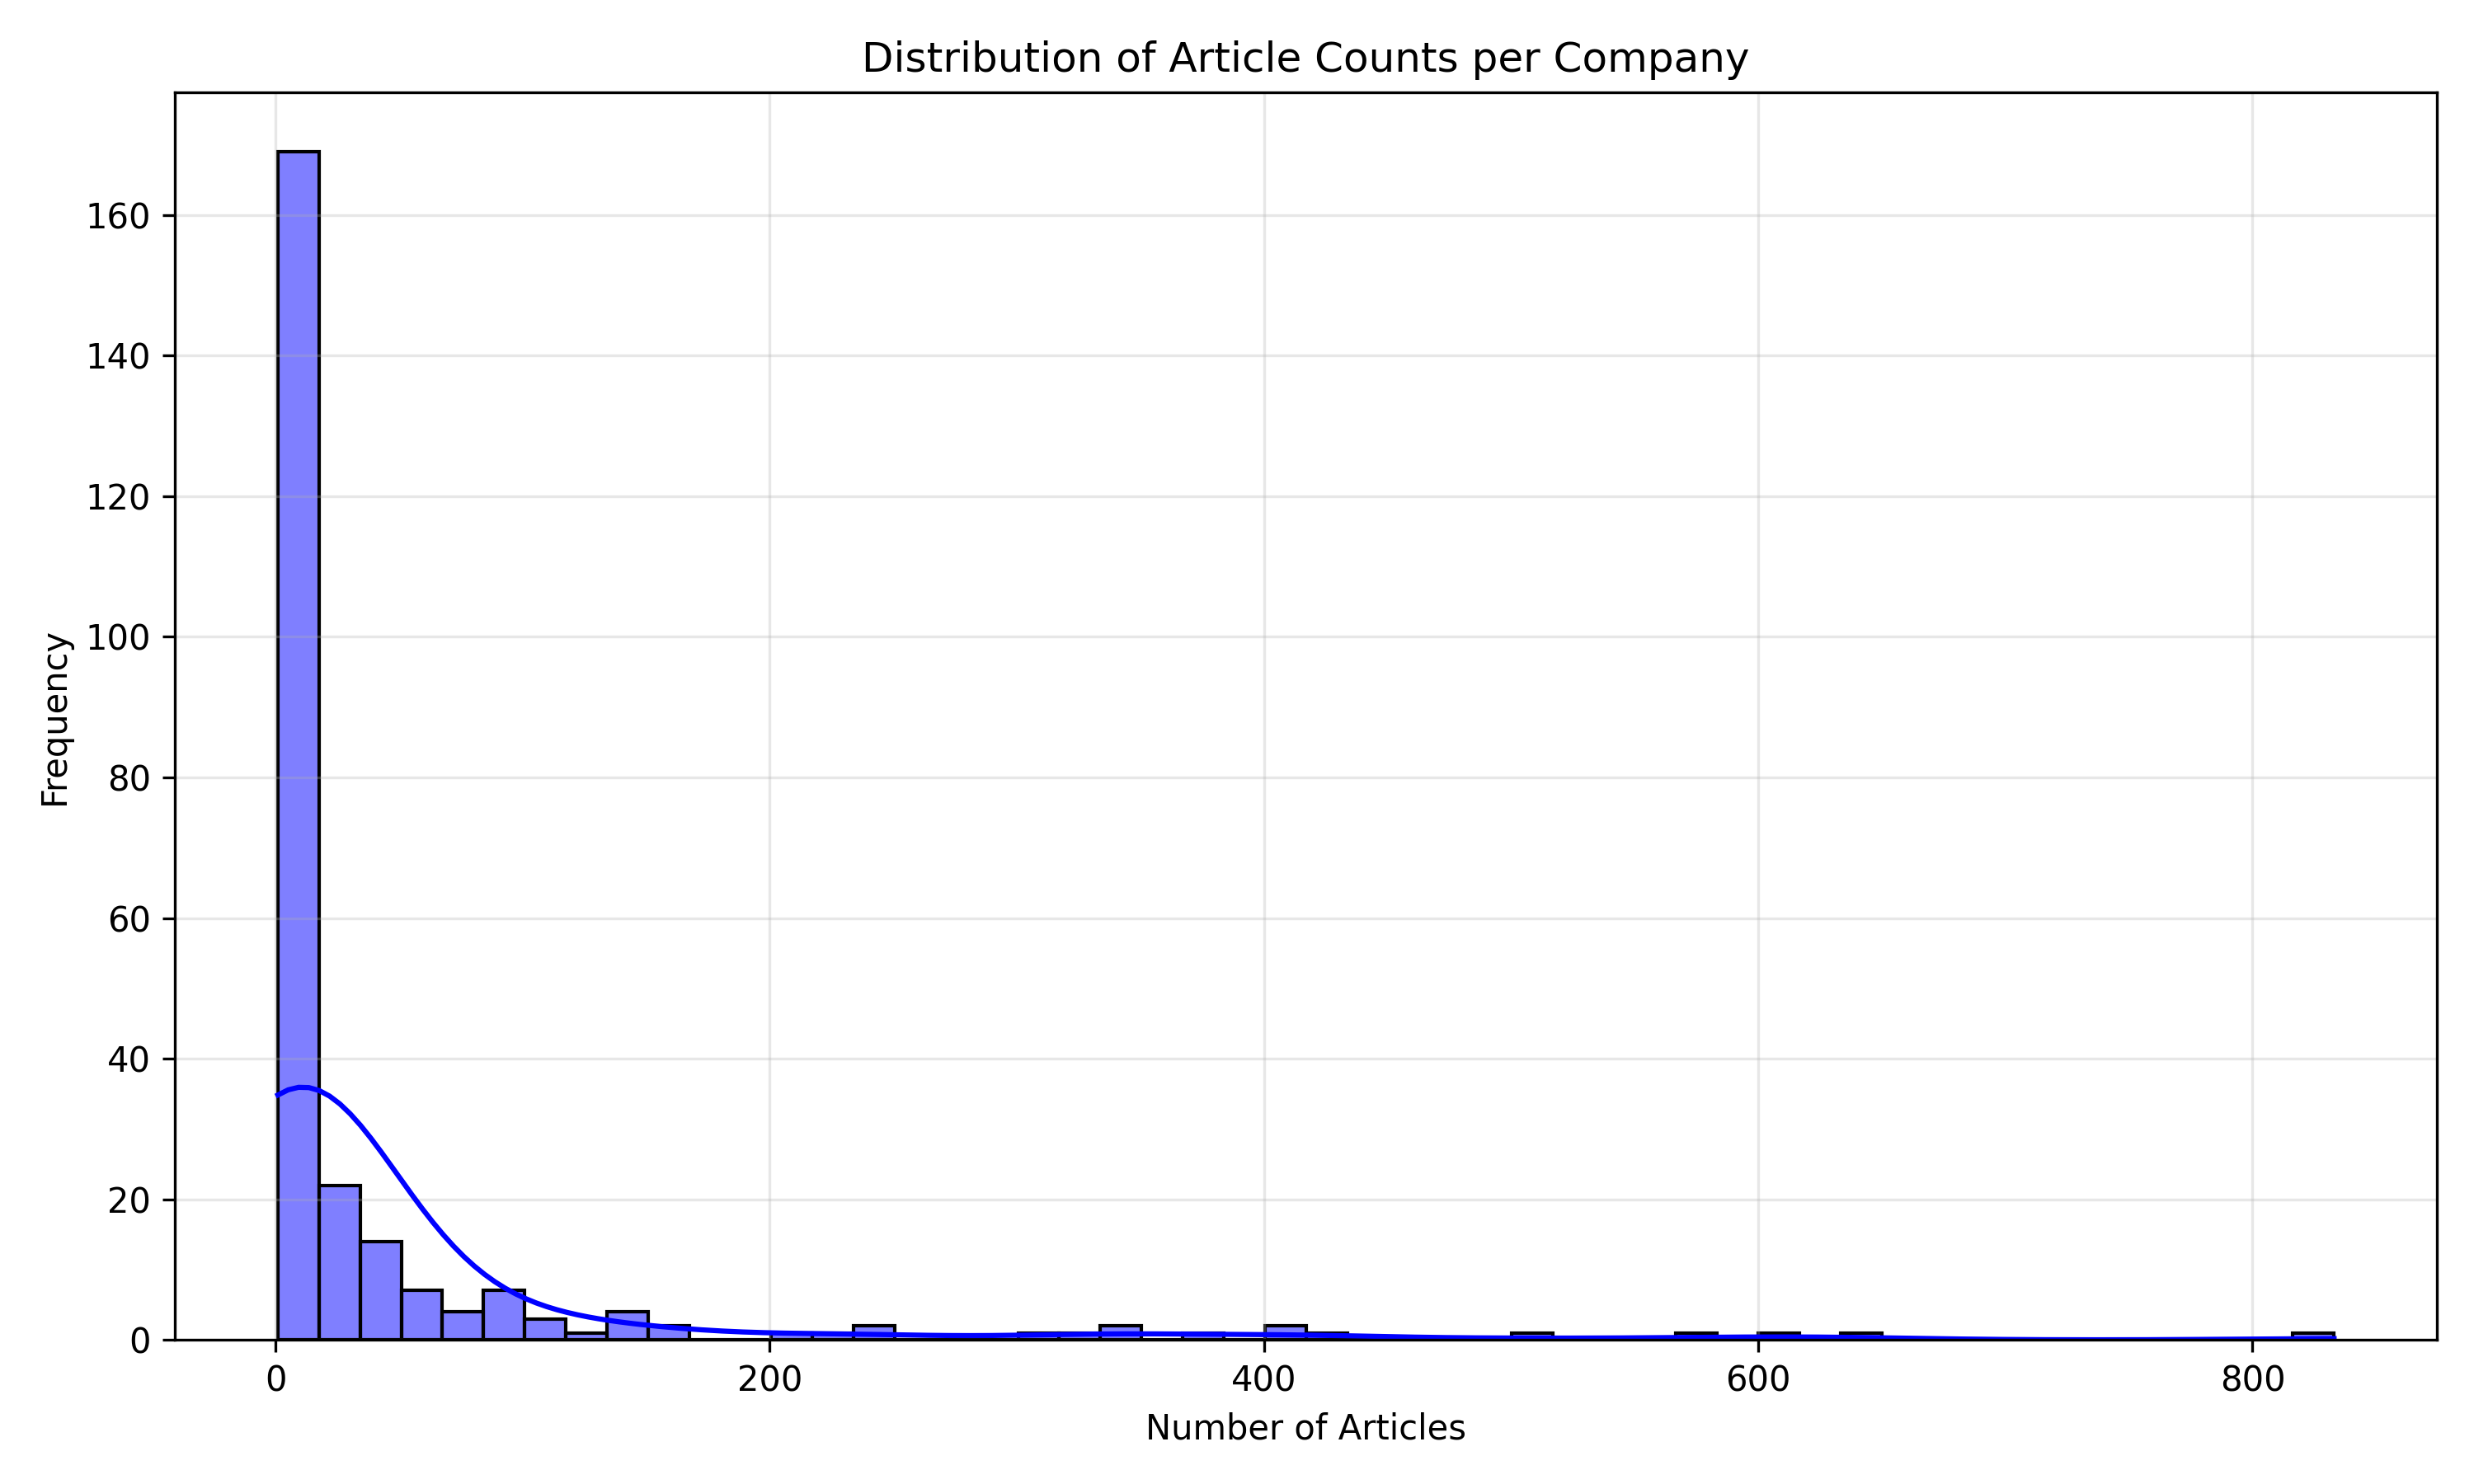
\includegraphics[width=\linewidth]{article_count_distribution.png}}
\caption{Distribution of article counts per company. The long tail motivates stratified sampling to avoid coverage-driven bias.}
\label{fig:article_count_distribution}
\end{figure}

\begin{figure}[htbp]
\centerline{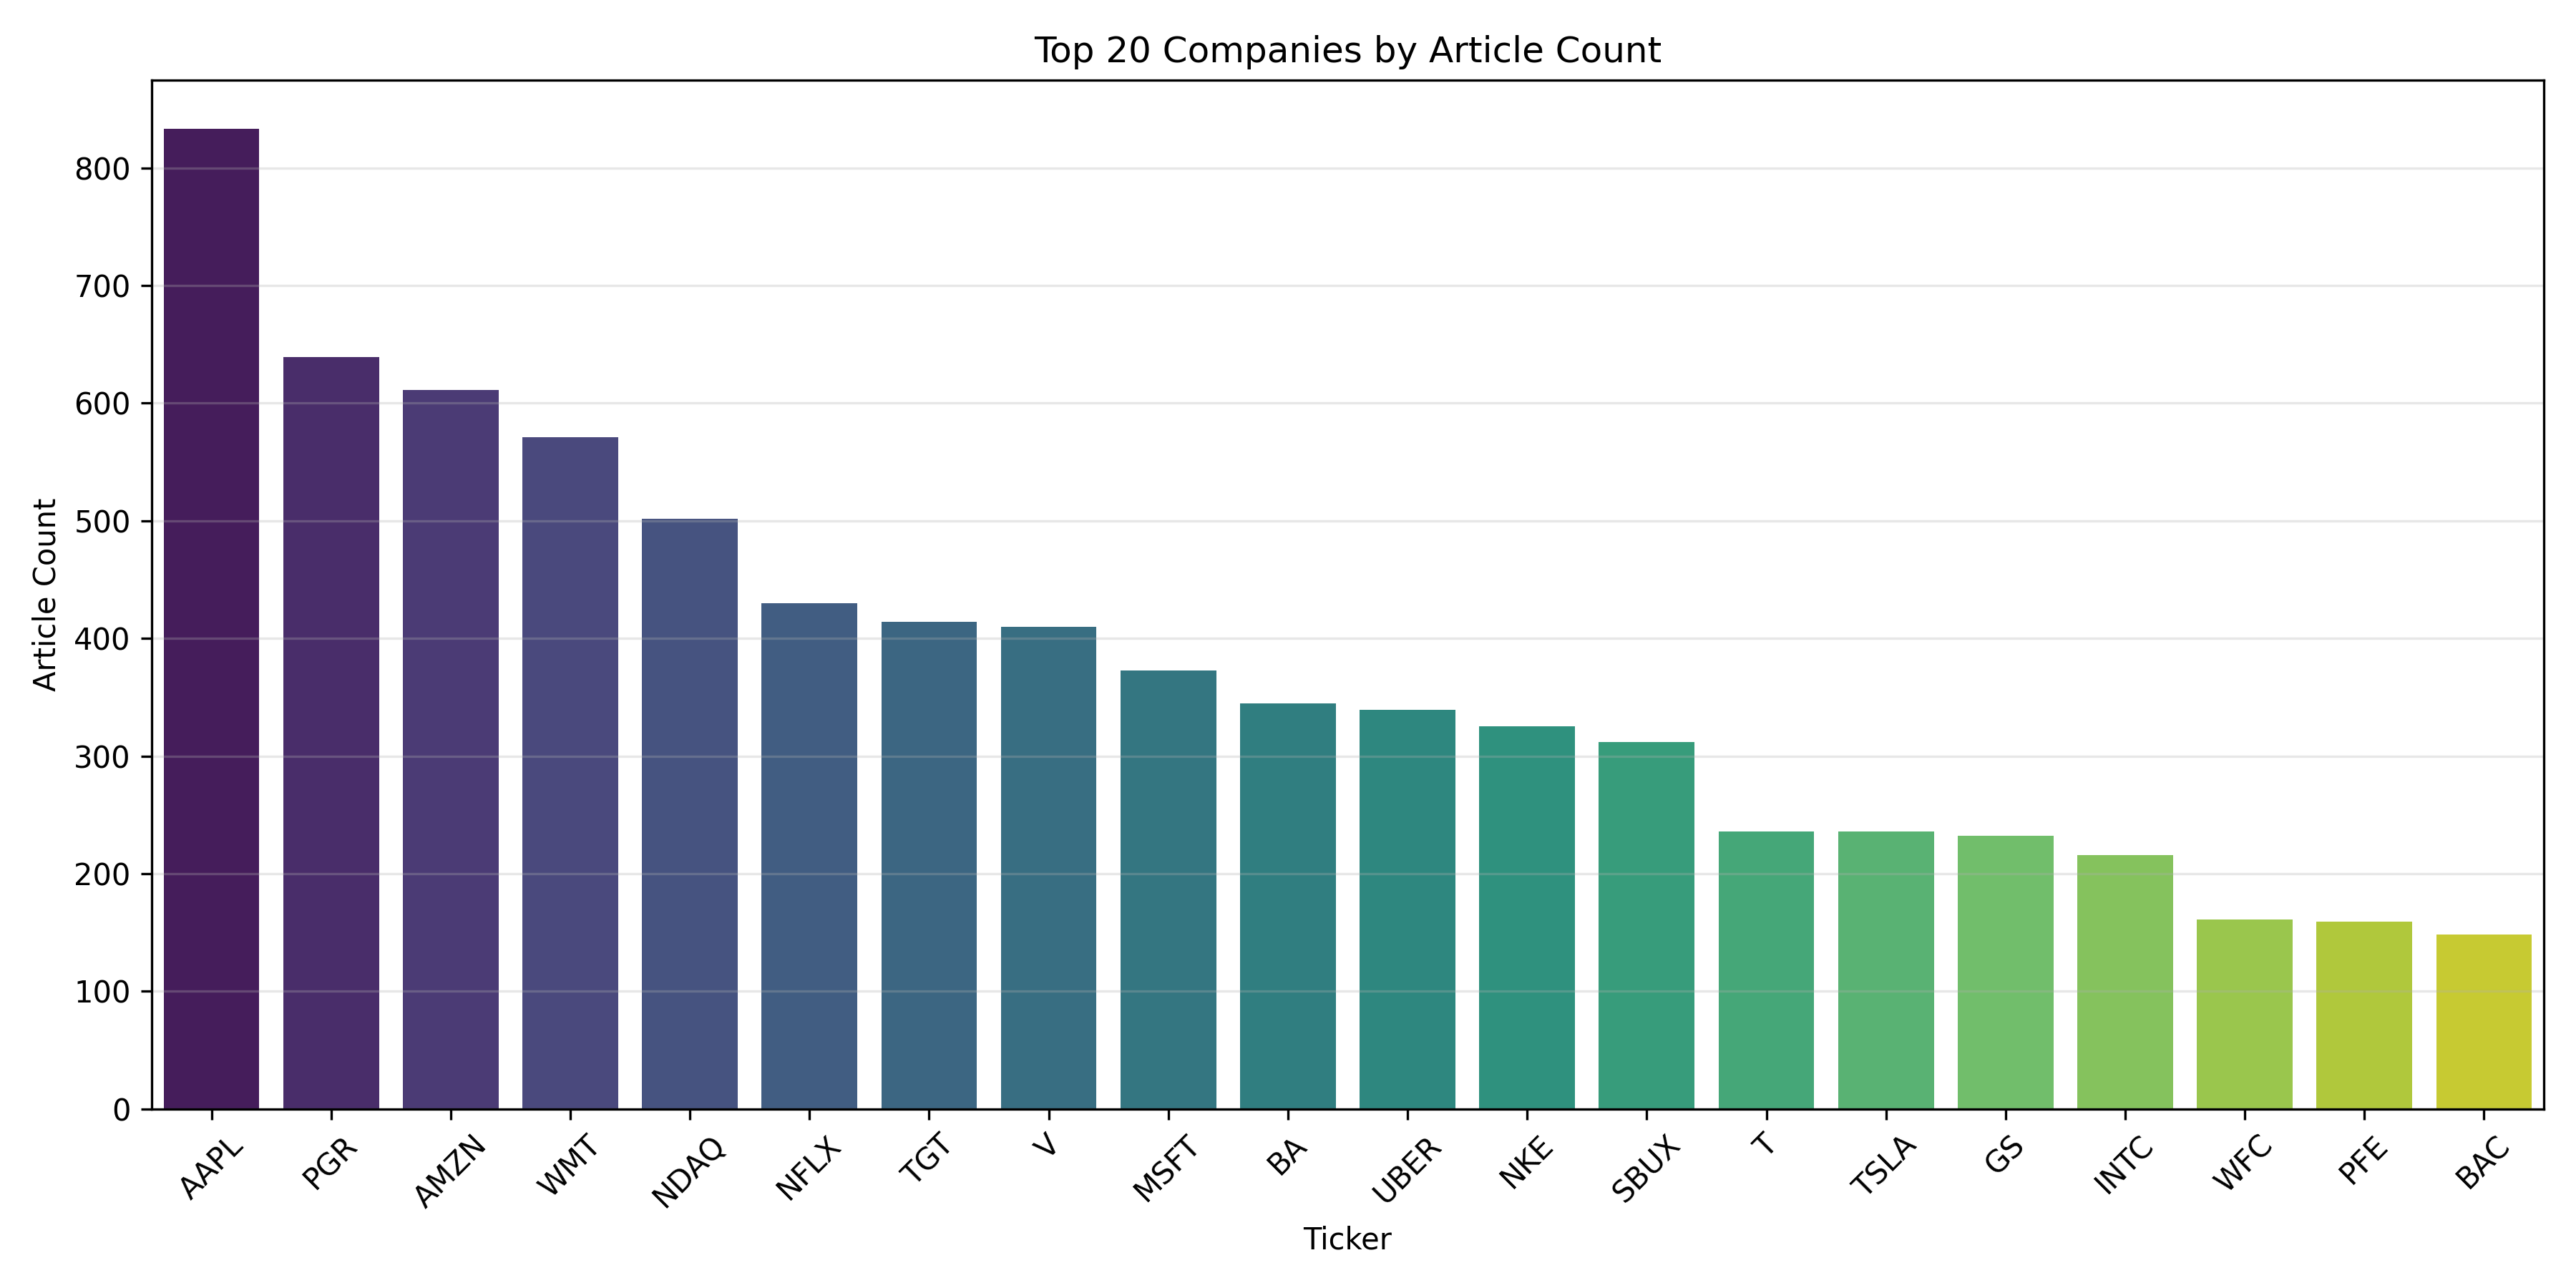
\includegraphics[width=\linewidth]{top_20_articles.png}}
\caption{Top 20 firms by article count in the retained sample.}
\label{fig:top20_articles}
\end{figure}

\subsection{Relevance Filtering and Annotation}
Keyword matching is not enough for firm targeting (e.g., ``Apple'' is not always the company). We therefore apply a two-stage relevance pipeline: (i) title-based pre-filtering that retains only articles with the company name in the title (company names, not tickers), and (ii) a supervised relevance classifier trained on manual annotations. The held-out test set for manual annotation is kept completely separate from training.

Our base classifier is DeBERTa-v3 fine-tuned for binary classification using article titles. The first model, trained on 750 labeled articles, achieved high recall but insufficient precision. We then expanded the training data via semi-supervised mining: running the model on a large unlabeled pool and adding only high-confidence predictions ($p_{rel} \ge 0.92$ for relevant, $p_{rel} \le 0.05$ for irrelevant). This expanded set increases precision and reduces false positives. An ensemble of model variants further improves precision, and the operating threshold is selected via a sweep to meet a target of precision $\ge 0.90$.

\subsection{Stance Scoring}
Stance is computed using the NewsMTSC model for target-dependent stance. For each qualifying article we obtain probabilities for positive, negative, and neutral stance. The baseline specification retains only high-confidence outputs (prob >= 0.9), and we report sensitivity to lower thresholds (0.6 and 0.0). Daily firm-level stance is the average across articles on that day:
\begin{equation}
\text{stance}_{i,t} = \frac{1}{N_{i,t}} \sum_{a \in A_{i,t}} (p^{+}_{a} - p^{-}_{a})
\end{equation}
where $A_{i,t}$ is the set of high-confidence articles for firm $i$ on day $t$ and $N_{i,t}$ is the count. We also construct article volume and coverage mix covariates to separate tone shifts from coverage shifts.

\subsection{Market Alignment and Controls}
The stance series is aligned to firm-day market outcomes: daily returns, S\&P 500 index returns, and VIX. We also log-normalize article volume in regressions. This alignment yields the panel used across the RQ1--RQ3 specifications.

\section{Methodology}
This section groups the empirical strategy into three layers: (i) structural shifts around the 2020 shock, (ii) stance-return linkage, and (iii) time-series dynamics and event studies.

\subsection{RQ1: Stance Shift Around the 2020 Shock}
We test for a structural shift in stance using a pre/post specification with firm fixed effects:
\begin{equation}
\text{stance}_{i,t} = \alpha_i + \beta \cdot Post_t + \gamma' X_{i,t} + \varepsilon_{i,t}
\end{equation}
where $Post_t$ equals 1 after January 2020 (post period: 2020--2025; pre: 2015--2019) and $X_{i,t}$ includes article volume and VIX. If pre-period means are not comparable, we implement Synthetic Control DiD (SCDiD) or use an interrupted time-series specification with level and trend shifts.

\subsection{RQ2: Returns Shift Around the 2020 Shock}
The returns analogue mirrors the stance regression, with returns as the outcome and market controls added:
\begin{equation}
return_{i,t} = \alpha_i + \beta \cdot Post_t + \gamma' X_{i,t} + \varepsilon_{i,t}
\end{equation}
where $X_{i,t}$ includes index returns and VIX to absorb market-wide shocks.

\subsection{RQ3: Stance-Return Linkage}
We test the direct stance-return relationship using next-day returns:
\begin{equation}
return_{i,t+1} = \alpha_i + \beta \cdot \text{stance}_{i,t} + \gamma' X_{i,t} + \varepsilon_{i,t}
\end{equation}
To test whether the stance-to-return sensitivity changes post-2020, we use a triple interaction:
\begin{equation}
return_{i,t} = \alpha_i + \beta (Post_t) + \gamma \text{stance}_{i,t} + \delta (Post_t \times \text{stance}_{i,t}) + \theta X_{i,t} + \varepsilon_{i,t}
\end{equation}
where the interaction $Post_t \times \text{stance}_{i,t}$ captures post-shock amplification of the stance-return channel.

\subsection{Time-Series Dynamics and Event Studies}
We estimate VARs on (stance, returns) to capture bidirectional dynamics and compute impulse response functions. Granger causality tests evaluate whether past stance improves return forecasts beyond past returns, and whether the reverse also holds. We also test for autocorrelation in stance using ARIMA models, which motivates lagged stance controls.

As a non-parametric check, we run event studies around large stance jumps (e.g., >2 SD from a rolling mean) and compute abnormal returns in short windows around those events.

\subsection{Robustness and Sensitivity}
We perform numerous robustness checks: alternative stance aggregation (median, winsorized means), different confidence thresholds, exclusion of low-coverage firm-days, placebo pre/post cutoffs, and treatments that control for article topical composition. We also test sensitivity to training-test splits for the relevance classifier and manual annotation thresholds.

\section{Identification, Validity, and Robustness}
We address three main threats. First, macro shocks may move both coverage and prices; we control with index returns and VIX. Second, article volume differs widely across firms; we include volume covariates and run trimmed samples. Third, parallel trends may not hold; we use pre-trend checks, placebo cutoffs, and SCDiD when needed.

Robustness checks include alternate stance thresholds (0.9, 0.6, 0.0), alternative aggregation (mean vs median), lagged stance controls, sector controls, and quantile regressions to test for tail effects in returns.

\section{Conclusion and Next Steps}
This draft provides a full narrative of the project to date: why the 2020 shock matters, how we build a target-dependent stance signal, and how we test for structural changes and market effects. Next steps include finalizing the firm panel, completing the relevance classifier evaluation, computing the daily stance series, and running the full RQ1--RQ3 specifications with robustness tables and figures.

\bibliographystyle{IEEEtran}
\begin{thebibliography}{99}
\bibitem{hamborg2021} F. Hamborg and K. Donnay, ``NewsMTSC: Target-dependent stance classification in news articles,'' EACL, 2021.
\bibitem{haroon2020} O. Haroon and S. A. Rizvi, ``COVID-19: Media coverage and financial markets behavior,'' Finance Research Letters, 2020.
\bibitem{blajer2024} M. Blajer-Golebiewska, A. Honecker, and K. Nowak, ``Investor sentiment response to COVID-19: A sectoral analysis,'' North American Journal of Economics and Finance, 2024.
\bibitem{news2024} ``News and markets in the time of COVID-19,'' Journal of Financial and Quantitative Analysis, 2024.
\bibitem{davis2020} S. Davis, S. Hansen, and C. Seminario, ``Firm-level risk exposures and stock returns in the wake of COVID-19,'' NBER, 2020.
\bibitem{costola2023} M. Costola, M. Nofer, O. Hinz, and L. Pelizzon, ``Machine learning sentiment analysis, COVID-19 news and stock market reactions,'' Research in International Business and Finance, 2023.
\bibitem{bai2023} Z. Bai, Q. Han, J. Pan, and R. Zhang, ``Financial market sentiment and returns,'' Finance Research Letters, 2023.
\bibitem{xu2024} H. Xu, ``News bias in financial journalists' social networks,'' Journal of Accounting Research, 2024.
\end{thebibliography}

\end{document}
